% Тут используется класс, установленный на сервере Papeeria. На случай, если
% текст понадобится редактировать где-то в другом месте, рядом лежит файл matmex-diploma-custom.cls
% который в момент своего создания был идентичен классу, установленному на сервере.
% Для того, чтобы им воспользоваться, замените matmex-diploma на matmex-diploma-custom
% Если вы работаете исключительно в Papeeria то мы настоятельно рекомендуем пользоваться
% классом matmex-diploma, поскольку он будет автоматически обновляться по мере внесения корректив
%

% По умолчанию используется шрифт 14 размера. Если нужен 12-й шрифт, уберите опцию [14pt]
\documentclass[14pt]{matmex-diploma}
%\documentclass{matmex-diploma-custom}
\usepackage{amssymb}
\usepackage{amsmath}
\usepackage{multirow}
\usepackage{graphicx}
\usepackage{enumitem}
\usepackage{subcaption}
\usepackage{pgfplots}
\usepackage{csvsimple}
% \usepackage{floatrow}
% \usepackage{siunitx}
%\usepackage{wrapfig}
\usepackage{tikz} % To generate the plot from csv


\pgfplotsset{compat=newest} % Allows to place the legend below plot
\usepgfplotslibrary{units} % Allows to enter the units nicely


\begin{document}
\filltitle{ru}{
    chair              = {Кафедра Системного Программирования},
    title              = {Рандомизированный алгоритм при обработке данных ультразвуковых исследований},
    % Здесь указывается тип работы. Возможные значения:
    %   coursework - Курсовая работа
    %   diploma - Диплом специалиста
    %   master - Диплом магистра
    %    bachelor - Диплом бакалавра
    type               = {bachelor},
    position           = {студента},
    group              = 444,
    author             = {Сенин Иван Игоревич},
    supervisorPosition = {д.\,ф.-м.\,н., профессор},
    supervisor         = {О.\,Н. Граничин},
    reviewerPosition   = {аспирант},
    reviewer           = {К.\,И. Тюшев},
    chairHeadPosition  = {д.\,ф.-м.\,н., профессор},
    chairHead          = {А.\,Н. Терехов}
   university         = {Санкт-Петербургский Государственный Университет},
   faculty            = {Математико-механический факультет},
   city               = {Санкт-Петербург},
   year               = {2016}
}
\filltitle{en}{
    chair              = {Department of Software Engineering},
    title              = {Randomised algorighm in ultrasonic investigation precessing},
    author             = {Ivan Senin},
    supervisorPosition = {professor},
    supervisor         = {Oleg Granichin},
    reviewerPosition   = {postgraduate},
    reviewer           = {Kirill Tyushev},
    chairHeadPosition  = {professor},
    chairHead          = {Andrey Terekhov},
    % city              =   {Saint Petersburg}
}
\maketitle
\tableofcontents
% У введения нет номера главы
\setcounter{section}{0}
\section*{Аннотация}
Ультразвуковая томография нашла широкое применение в медицинской практике. По мере развития технологий стало возможным использование большего количества датчиков для получения более качественного изображения. Кроме того, для хорошей фокусировки необходима высокая частота дискретизации получаемого сигнала, что ведёт к большому объему обрабатываемой информации.  Однако, характер получаемых при томографии изображений имеет разреженный профиль, из чего следует, что необходимое для восстановления количество информации очень мало. В то же время имеется значительная избыточность данных, что оставляет возможность для разработки более оптимальной технологии сбора и анализа в процессе томографического исследования. В этой работе предложен прототип эффективной технологии по сбору и реконструкции изображений ультразвуковой томографии, основанной на принципах рандомизированных алгоритмов, которая позволяет сократить время исследования без потерь в качестве. 


\section{Введение}

\subsection{Актуальность}
Ультразвуковая томография по качеству и разрешающей способности достигла сопоставимого с МРТ уровня и активно применяется для исследования мягких тканей \cite{hopp2014breast}.
Преимуществами УЗИ являются относительно низкая стоимость оборудования и обслуживания, безопасность для организма, неинвазивность техники исследования. \\

Для повышения качества и разрешающей способности получаемого в ходе исследования изображения требуется увеличение количества используемых датчиков и частоты дискретизации сигнала. Всё это ведёт к значительному увеличению объема передаваемых данных, что усложняет как производственный процесс, так и проведение диагностики. Кроме того особенности проведения исследования допускают наличие помех и искажений \cite{shannon_th}. \\

Опухоли преимущественно имеют более высокую скорость прохождения ультразвука, чем окружающие ткани. Это делает возможным реконструкцию плотностей тканей в исследуемой зоне с помощью уравнений с участием предполагаемых путей распространения сигнала и временем его прибытия на датчики кругового массива (\textit{travel time tomography}) \cite{quan2007sound}. Современные системы основаны именно на таком подходе и получили применение в диагностике рака молочных желез \cite{hormati2010robust}\cite{schreiman1984ultrasound}. \\

Для метода томографии travel-time типична квадратичная от числа сенсоров зависимость получаемых ``сырых'' данных для анализа: последовательно с каждого датчика пускается ультразвуковой импульс, который принимают остальные $k-1$ сенсоров. Это приводит к серьезному повышению требований к вычислительной части устройства томографа, а также к увеличению времени обработки: современные методы реконструкции работают итеративно с временной сложностью итерации $O(N\log N)$ \cite{chen2012compressive}. \\

На настоящий момент использование ультразвуковой томографии осложнено высокими требованиями к вычислительному комплексу и временем на обработку \cite{ozmen2014ultrasound}. Уменьшение объема данных позволит эффективно использовать FPGA вычислители для задач определения времени прибытия сигнала на датчик и последующей реконструкции изображения. Compressive Sensing также позволит сократить время на сбор данных путем уменьшения количества производимых проекций, что частично сократит зашумление данных из-за колебаний пациента в процессе обследования.


\subsection{Обзор литературы и ключевые работы в области}

\subsubsection{Travel-time томография} \label{sec:travel_times_descr}
Техника томографии по времени прибытия сигнала уже хорошо изучена и освещена в работах \cite{Kunyansky2012111}, \cite{quan2007sound}, \cite{hopp2014breast}. В том числе рассмотрены алгоритмы в отношении устойчивости к присутствию шума \cite{hormati2010robust}. Далеко не последнюю роль в реконструкции изображения играет точное определение времени прибытия сигнала \cite{li2009improved}. Общий процесс обработки данных томографии времени прибытия показан на рис.\ref{fig:us_process}.
\begin{figure}[h]
\centering
    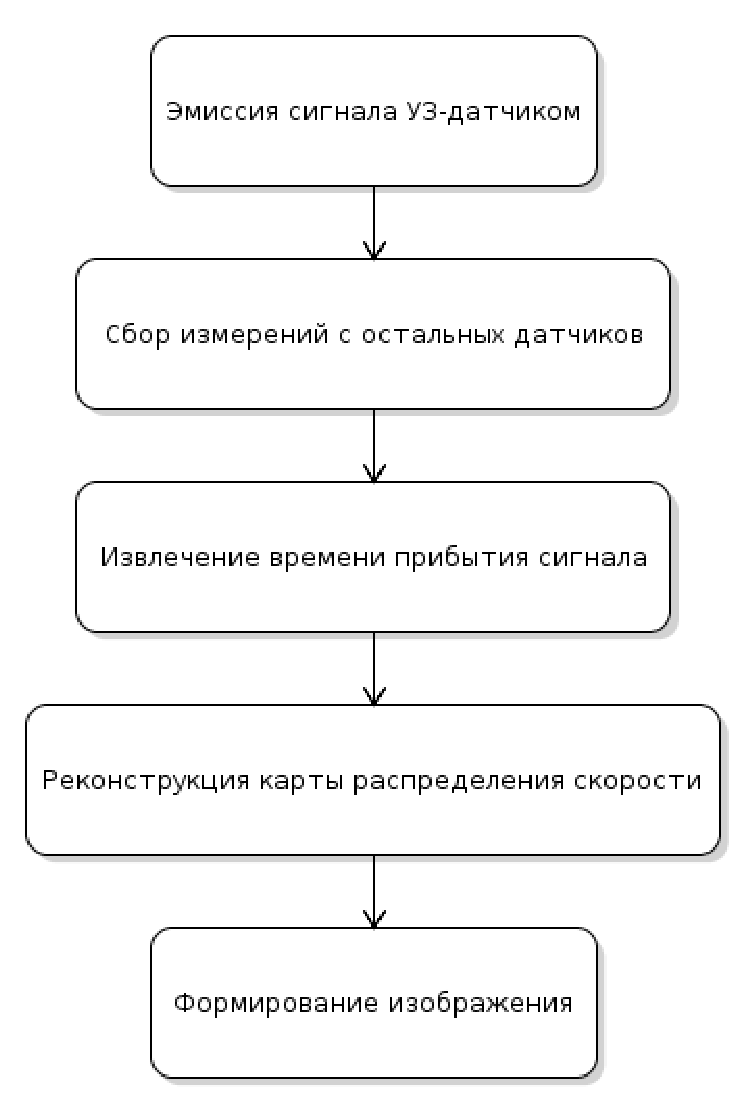
\includegraphics[width=0.5\textwidth]{pics_eps/us_process.eps}
    \caption{\small Общий вид процесса ультразвуковой томографии времени прибытия}
    \label{fig:us_process}
\end{figure}
Основная цель акустической томографии -- восстановить параметры неизвестной среды изучая характеристики распространения звука в ней. Во-первых, для этого требуется точная модель, хорошо описывающая лежащую в её основе физическую систему, и, во-вторых, высокоточные измерения. Тогда решением обратной задачи составляется оценка неизвестной модели. Корректность физической модели, точность измерений и выбор метода решения обратной задачи имеют прямое влияние на качество реконструкции. \\

Распространение энергии акустического сигнала в неоднородной среде хорошо описывается дифференциальным уравнением в частных производных второго порядка
$$\nabla^2p(r,t) - \frac{1}{F^2(r)}\frac{\partial^2p(r,t)}{\partial t^2} = s(r,t)$$
где $p(r, t)$ --- давление в $r$ в момент времени $t$, $F(r)$ --- неизвестная модель распространения скорости и $s(r,t)$ --- первоначальный сигнал. Зная исходный сигнал $s(r, t)$, решая обратную задачу, находим модель $F(r)$, которая лучше всего описывает измерения $p(r,t)|_{\Omega}$, записанные на известных границах $\Omega$.\\

Моделирование прямой задачи по уравнению распространения волны вычислительно весьма трудоемко, вследствие чего в travel-time томографии используются принципы геометрической акустики. При предположении, что частота звукового сигнала достаточно высока, можно найти его путь распространения используя принципы Ферма \cite{schuster1904introduction}. Тогда обратная задача состоит в реконструкции распределения скорости звука $F(r)$ исходя из времени сигнала в пути, получаемое с показаний датчиков. Следует отметить, что в отличии от задач томографии с помощью рентгена, где сигнал распространяется по прямой, распространение ультразвукового сигнала в неоднородной среде происходит иначе и зависит от распределения скорости.\\

В то время как акустическая \textit{томография по времени прибытия} сигнала берет свои корни из сейсмологии\cite{dines1979computerized}, на сегодняшний день уже множество исследований показало, что ультразвуковая томография имеет большой потенциал в области диагностирования рака груди \cite{duric2007detection}. \\

\textbf{Постановка обратной задачи по реконструкции изображения}\\
Время сигнала в пути от передатчика к приемнику вдоль траектории его распространения можно представить как
\begin{equation}\label{eq:time_of_fl_cont}
Y = \int_\Gamma \frac{1}{F(r)}ds,
\end{equation}
где $Y$ --- время прибытия сигнала, $\Gamma$ --- путь его распространения, $F(r)$ --- скорость звука в точке $r$. Следует заметить, что проходимый сигналом путь $\Gamma$ зависит от распределения скорости в среде $F(r)$. Существует нелинейная зависимость между временем сигнала в пути и скоростью звука в среде. Можно представить уравнение \eqref{eq:time_of_fl_cont} в дискретной форме, наложив сетку на интересующую для восстановления область с константными значениями скорости звука в клетках общим количеством $N$ ячеек:
\begin{equation}\label{eq:2}
Y = A(F)\cdot F,
\end{equation}
где $F$ --- вектор $[N\times 1]$, представляющий интересующее распределение скоростей, а $A(F)$ --- матрица $[M\times N]$, представляющая путь, по которому проходит сигнал и $t$ --- вектор $[M\times 1]$, содержащий время прибытия сигнала, полученное анализом показаний с датчиков. Так имея в установке $k$ датчиков, получаем $M = k\cdot (k-1)$ всевозможных траекторий кратчайшего прохождения сигнала. \\

Целью обратной задачи является нахождения такой оценки распределения скоростей \^{m}, которая лучше всего описывает время прохождения пути сигналом в уравнении \eqref{eq:2}. Одним из традиционных алгоритмов решения является метод LASSO с нормой $\ell_1$ и вариацией для регуляризации \cite{hormati2010robust}. Тогда задача представляется как задача минимизации
\begin{equation}
\label{eq:lasso}
\min_F \| A(F) \cdot F - Y \|_2^2 + \lambda \| \Psi^T F \|_1 + \lambda_{TV} TV(F),
\end{equation}
где $\Psi$ --- некоторый базис, переводящий $F$ в разреженное представление и $\lambda, \lambda_{TV}$  --- положительные весовые коэффициенты.



\subsubsection{Compressive Sensing} \label{sec:cs_description}
С начала третьего тысячелетия объемы получаемой и обрабатываемой информации существенно возросли. Главным образом это связано с увеличением размерностей передаваемых сигналов (от одномерных ``1-D'' к дву- и  трех- мерным). При этом рост данных происходит по экспоненциальному закону относительно размерности. Также в современных системах происходит постоянный пост требований к частоте измерений (теорема Шеннона-Найквис\-та-Котель\-никова). Все это влечет необходимость сжатия данных для хранения и пересылки, стоимость суммарной обработки оказывается очень дорогостоящей\cite{граничин2010рандомизация}.
Интересующую информацию можно представить как $x \in \mathbb{X}$, которую предстоит получить с помощью набора наблюдений $y \in \mathbb{Y}$. Между $x$ и $y$ существует закономерность явления $\Phi:\mathbb{X}\to\mathbb{Y}$. В случае, когда $\Phi$ обратим и при линейной зависимости, известно, что $x = \Phi^{-1}y $. Для систем реального мира более типичным является случай, когда результаты наблюдений подвержены различным помехам \[y = \Phi x + \xi\]
При значительных помехах задача решается статистически, используя $m >> N$ при $x \in \mathbb{R}^N$. Известно, что такая задача о восстановлении $x$ может быть решена даже в случае нецентрированных коррелированных помех за счет случайного выбора матрицы $\Phi$ \cite{granichin2004linear}. Установлено, что рандомизация позволяет не только устранить эффект смещения, но и уменьшить количество итераций алгоритма оценивания $x$ \cite{граничин2003рандомизированные}. \\

На практике интересно рассмотреть возможности восстановления $x \in \mathbb{R}^N$ при $m << N$, что, очевидно, невозможно в общем случае. Однако, оказалось, что задача может быть решена с достаточной точностью, при выполнении некоторых условий \cite{donoho2006compressed}. Подобная парадигма получения и восстановления данных называется \textit{Compressive Sensing} или \textit{Опознание со сжатием}. \\

Постановка задачи о получении и восстановлении данных в общем виде выглядит следующим образом. Пусть $x$ --- интересующая информация. Она проявляется себя через сигнал $f = \Psi x$. С помощью каких-либо приборов регистрирования получают наблюдения $y = A f$. По ним исследователю необходимо восстановить исходную информацию $x$, формируя оценки \^{x}. \\

\textbf{Проектирование матрицы измерений}\\

Получение $m << N$ наблюдений можно представить как скалярное произведение с множеством некоторых векторов $\{a_i\}_{i=1}^m$, или умножением на матрицу размерности $m\times N$: $y= A f$. Тогда из постановки задачи следует $y=A f = A \Psi x = \Phi x$, где $\Phi$ --- матрица $m \times N$. \\

Необходимыми и достаточными условиями, предъявляемыми теорией \textit{опознания со сжатием}, являются:
\begin{itemize}
\item сигнал $f$ является $s-$разреженным: \\существует такой базис $\Psi$, что $f = \sum_{j=1}^N x[j] \psi_j$, где только $s$ коэффициентов $x[j]\neq 0$
\item выполняется ``свойство ограниченной изометрии'' (Restricted Isometry Property, RIP):
$$\text{RIP}(\delta, m)= \sqrt{1 - \delta} \leq \frac{\| \Phi z \|_2}{\| z\|_2} \leq \sqrt{1 + \delta},$$ 
где $\delta \in (0,1)$ и $z$ --- произвольный ненулевой $m$-разреженный вектор.

\item свойство ``некогерентности'' (малой взаимной зависимости) $A$ и $\Psi$:
$$\mu (A, \Psi) = \sqrt{N} \max_{i,j}\frac{|\langle a_i, \psi_j\rangle |}{\| a_i\|_2}.$$
Установлено, что случайные матрицы $A$ с высокой вероятностью некогерентны с любым фиксированным базисом $\Psi$.
Из \cite{candes2007sparsity} следует достаточное условие для высокой вероятности точного восстановления $s-$разреженных векторов по m наблюдениям:
\begin{equation}m \geq c \mu (A,\Psi)^2 s \log{N}, \end{equation}
где $c$ --- некоторая положительная постоянная.
\end{itemize}

В \cite{cande2008introduction} указывается замечание, что на практике часто достаточно $m\approx 4s$. Также известно, что условие $\text{RIP}(\delta, 2s)$ является недостаточным для восстановления в присутствии помех или если в сжимаемом сигнале $N - s$ компоненты малы, но не равно нулю. Для робастности же достаточным условием будет $\text{RIP}(\delta, 3s)$. Явное построение матрицы измерений $A$: $\Phi = A\Psi$ требует проверки условия RIP для каждой комбинации положений $s$ ненулевых компонент вектора $z$ длиной $N$ (т.~е. $C_N^s$). Однако, оказывается, что случайная матрица $m \times N$ с элементами $a[i, j] \sim \mathcal{N}(0, \frac{1}{m})$ имеет следующие полезные свойства\cite{candes2006robust}:
\begin{itemize}
\item если $m \geq c_1 s \log{\frac{N}{s}}$ при $0 < \delta < 1$, тогда \\
$$\mathcal{P}\{A \in \text{RIP}(\delta, m)\} \geq 1 - 2e^{-c_2 m},$$
где $\mathcal{P}$ --- вероятность, $c_1,c_2 > 0$  --- малые постоянные, зависящие от $\delta$. И тогда, следовательно, $s-$разреженные сигналы длины $N$ могут быть восстановлены по $m << N$ измерениям с высокой вероятностью.
\item если матрица $A$, удовлетворяет указанным условиям, то и $\Phi = A\Psi$ также будет являться матрицей с независимо нор\-маль\-но-рас\-пре\-де\-лен\-ными элементами, что влечет $\Phi \in \text{RIP}(\delta ,m)$ с той же вероятностью и для любого ортонормированного базиса $\Psi$.
\end{itemize}

Для использования опознания со сжатием помимо проектирования матрицы измерений $A$ требуется разработать \textbf{алгоритм реконструкции сигнала}, задачей которого восстановить по $y \in \mathbb{R}^m$, матрице измерений $A$ и базису $\Psi$ сигнал $f \in \mathbb{R}^N$, или эквивалентное ему спектральное разреженное представление $x$.\\

При $m < N$ для $s$-разреженных сигналов имеется бесконечное число $x'$ : $\Phi x' = y$, т.~к. если $\Phi x = y \implies \Phi(X+r) = y$ для любого $r \in \text{Ker }\Phi$. Таким образом, алгоритм реконструкции должен найти вектор разреженного представления сигнала в $(N - m)$-размерном подпространстве $\mathcal{H}=\text{Ker }\Phi + x$.\\

\textbf{Методы решения обратной задачи}\\

Традиционным подходом в решении подобных обратных задач является поиск в $\mathcal{H}$ вектора с минимальной энергией (нормой)  $\ell_2$: $$ \hat{x} = \arg\!\min{\| x'\|_2} : \Phi x' = y,$$ или, что тоже самое, в форме метода наименьших квадратов
$$\hat{x} = \Phi^T (\Phi\Phi^t)^{-1}y.$$
Поскольку $\ell_2$ норма  отражает энергию сигнала, а не разреженность, результат будет содержать много ненулевых компонент. С задачей поиска разреженного решения хорошо справляется ``$\ell_0-$норма''. Однако, задача $\ell_0$ оптимизации невыпукла и относится к комбинаторному типу, процедуры ее решения, в общем случае, $NP$-сложные \cite{natarajan1995sparse}. Существует два подхода для приближенного решения таких задач: ``жадные'' стратегии оптимизации\cite{mallat1993matching} или переход к $\ell_1$-норме. Хорошо известно, что минимизация $\ell_1$ нормы способствует разреженности \cite{donoho2006most} и позволяет хорошо приближать разреженные сигналы используя только $m \geq c_1 s \log{\frac{N}{s}}$ случайных измерений \cite{donoho2006compressed}\cite{candes2006robust}. Это задача выпуклой оптимизации, сводимая к известной задаче линейного программирования ``выбор базиса'' (Basis Pursuit Denoising) \cite{chen2001atomic}, эффективные методы решения которого имеют временную сложность $\mathcal{O}(N\log{N/s})$ \cite{berinde2008practical}.\\

Техника обработки сигналов \textit{Compressive Sensing} может быть использована для решения проблемы передачи и обработки большого количества информации с массива датчиков. Этот метод уже успешно применяется в магнитно-резонансной томографии \cite{lustig2007sparse, lustig2008compressed}, а также в ультразвуковых исследованиях \cite{quinsac2010compressed}. Однако, данные, используемые для получения изображения в ультразвуковой томографии имеют иную природу, чем в классическом (B-mode) ультразвуковом исследовании, так как после замера сигнала из него извлекается время прибытия звуковой волны, с которой и происходит вся дальнейшая работа по реконструкции снимка. Также этот факт отличает ультразвуковую томографию от МРТ, где все необходимые для реконструкции данные получают уже в разреженном представлении.

\subsection{Предварительный пример}

В целях получения наилучшего изображения требуется большое количество датчиков и высокая частота дискретизации сигнала. Всё это ведёт к необходимости обработки серьезного объема данных. Оценить количество данных, поступающих непосредственно с датчиков можно как
\[ V = k^2  z  Y_{max} \nu,   \]
где $V$ --- общее число измерений сигнала, $k$ --- количество датчиков, $z$ --- количество исследуемых срезов, $Y_{max}$ --- время прохождения сигнала с учетом затухания эха, $\nu$ --- частота дискретизации. \\

Примером современного коммерческого ультразвукового томографа является The SoftVue\cite{roy2013breast}, который имеет следующие технические характеристики системы:
\begin{itemize}
\item Мастер сервер: 2 процессора quad-core Intel Xeon E5620, 192 ГБ ОЗУ
\item Сервер реконструкции: 2 процессора quad-core Intel Xeon E5620, 96 ГБ ОЗУ, 2 ГП Nvidia Tesla M2070
\end{itemize}

\begin{table}[h]
\centering
\begin{tabular}{ c | c | c | c }
    \hline
    \multirow{2}{*}{Частота дискретизации (МГц)} & \multicolumn{3}{c}{Число датчиков}  \\ \cline{2-4}
    & 256 & 512 & 1024 \\

    \hline
    10 & 0.21 & 0.86 & 3.44 \\
    12 & 0.26 & 1.03 & 4.13 \\
    14 & 0.30 & 1.20 & 4.81 \\
    \hline
\end{tabular}
\caption{\small Объем исходных данных ГБ за один срез в зависимости от числа датчиков в массиве и частоты дискретизации сигнала \cite{roy2013breast}.}
\label{table:datasize_ex}
\end{table}
Так в таблице \ref{table:datasize_ex} производители описали количество данных, получаемых с датчиков за один срез. На обработку такого среза при использовании только одного сервера для реконструкции требуется несколько минут, а при использовании всего вычислительного комплекса -- 20 секунд. Всего производится 70 срезов\cite{roy2013breast}. Таким образом время, затрачиваемое только лишь на вычисление томографических снимков, составляет приблизительно $23$ минуты.

\subsection{Результат (обзор)}

В ходе выполнения работы был разработан метод, позволяющий при разработке ультразвукового томографа внедрить в применяемые алгоритмы по сбору и обработке данных парадигмы опознания со сжатием. Эксперименты, проведенные на компьютерных моделях, показали состоятельность метода. В частности, даже в маломасштабной модели оказалось возможным сокращение используемых данных до 68\% от общего их объема.

\subsection{Структура работы}
В разделе \ref{sec:main_result} сначала демонстрируется факт разреженности восстанавливаемого сигнала, для чего было найдено подходящее трансформирующее кодирование. После чего рассматриваются различные варианты построения рандомизированной матрицы измерений, а также процесс реконструкции и архитектура программного решения. Далее приведены оценки необходимого для реконструкции объема данных при дальнейшем увеличении числа датчиков и разрешения снимка. Раздел \ref{sec:modeling} описывает проведенные эксперименты, где также анализируются полученные результаты. Подведение итогов проделанной работы происходит в разделе \ref{sec:concluding}.

\section{Постановка задачи}
Цели работы:
\begin{itemize}
  \item Исследовать возможность применения техники Compres\-sive Sen\-sing в задаче ультразвуковой томографии.
  \item Разработать рандомизированный алгоритм для сбора и обработки данных ультразвуковой томографии.
  \item Провести эксперименты на программной симуляции.
\end{itemize}

Для достижения поставленных целей необходимо:
\begin{enumerate}
\item Определить характеристики разреженности сигнала $s$, а также их изменения при дальнейшем увеличении разрешения получаемого изображения.
\item Для сбора измерений и последующего восстановления изображения следует спроектировать рандомизированную матрицу $A$. Согласно теории Compresive Sensing допустимы различные варианты ее построения.
\item Разработать модификацию алгоритма реконструкции томографического снимка.
\item На основании результатов программной симуляции выяснить эффективность полученного алгоритма.
\end{enumerate}



\section{Основной результат} \label{sec:main_result}
\subsection{Исследование разреженности изображения}
Для сравнения результатов алгоритмов реконструкции с исходной моделью в качестве метрики будем использовать среднеквадратичную ошибку (RMSE). Эта метрика уже была использована в работах по Compressive Sensing.


\subsubsection{Анализ характера разреженности сигнала} \label{sec:s_analysis}
Известно, что томографические снимки имеют разреженный характер. К категории эффективных трансформирующих преобразований, позволяющих привести восстановленную карту скоростей $F$ к разреженному представлению, относятся вейвлет-преобразования. Исследования Compressive Sensing в сфере МРТ показали эффективность вейвлета Добеши db6 \cite{lustig2007sparse}. \\
Пример использования вейвлета db6, примененного к результату реконструкции искусственной маломасштабной модели и результат преобразования $X = \Psi^{-1} F$ представлены на рис.~\ref{fig:speedmap} и рис.~\ref{fig:waveletted} соответственно.\\


\begin{figure}[!tbp]
    \centering
    \begin{minipage}[b]{0.45\textwidth}
        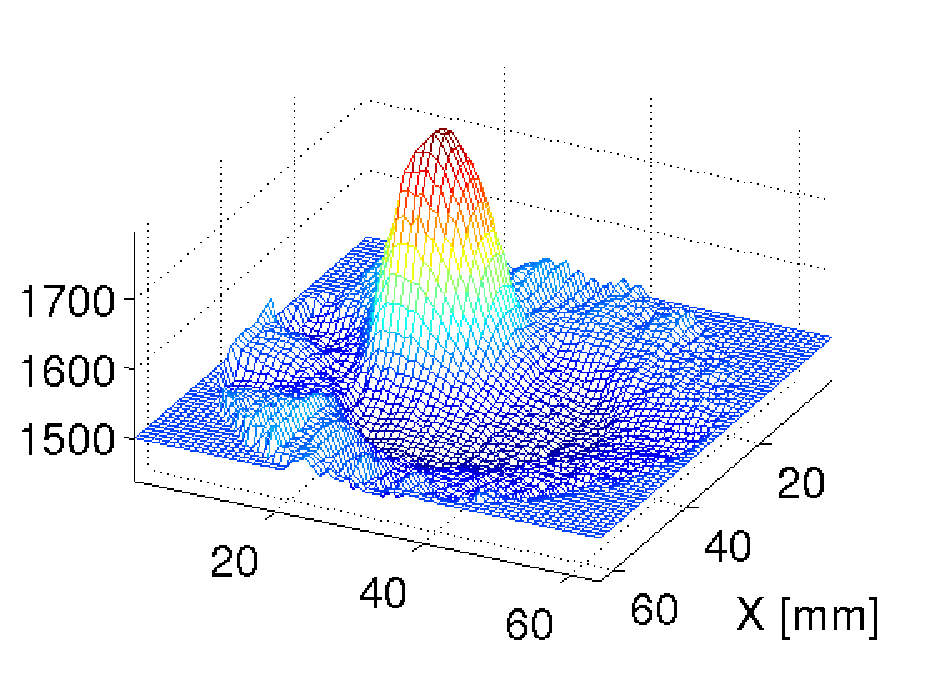
\includegraphics[width=\textwidth]{pics_eps/speed_map.eps}
        \caption{\small Карта скоростей, восстановленная из сигнала.}
        \label{fig:speedmap}
    \end{minipage}
    \hfill
    \begin{minipage}[b]{0.45\textwidth}
        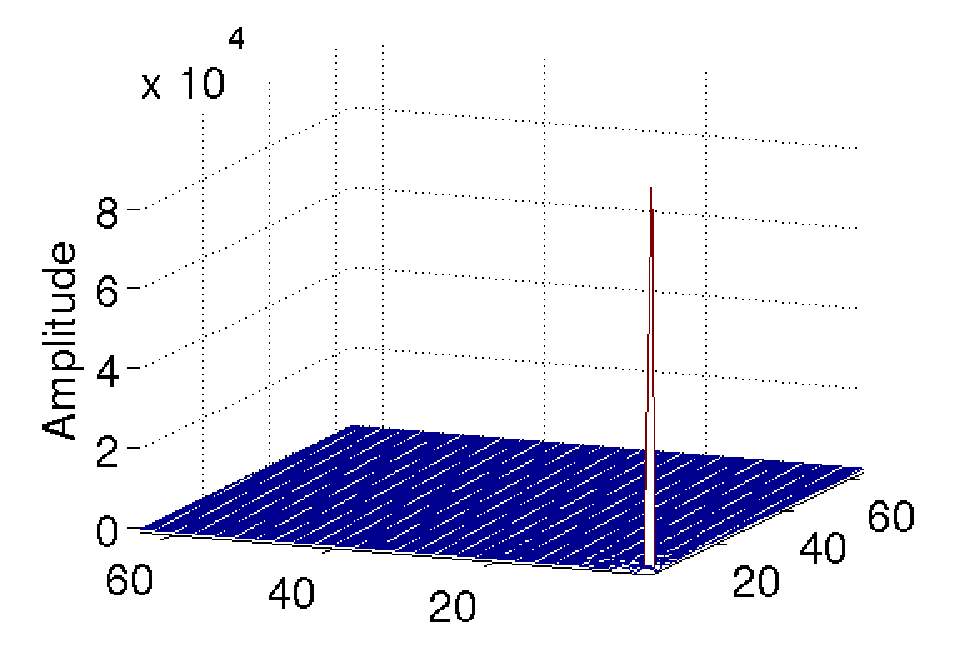
\includegraphics[width=\textwidth]{pics_eps/freq_domain.eps}
        \caption{\small Представление карты скоростей после вейвлет-преобразования.}
        \label{fig:waveletted}
    \end{minipage}
\end{figure}

\textbf{Анализ разреженности искусственной маломасштабной модели}\\

Согласно маломасштабной модели, общее количество коэффициентов составляет $N = 4096$.  Легко убедиться в разреженности сигнала: рис.~\ref{fig:used_coeff0} демонстрирует, что при использовании только лишь 100-200 коэффициентов происходит восстановление близкое к полному. \\

\begin{figure}[tbp]
  \centering
  \begin{minipage}[b]{0.8\textwidth}
    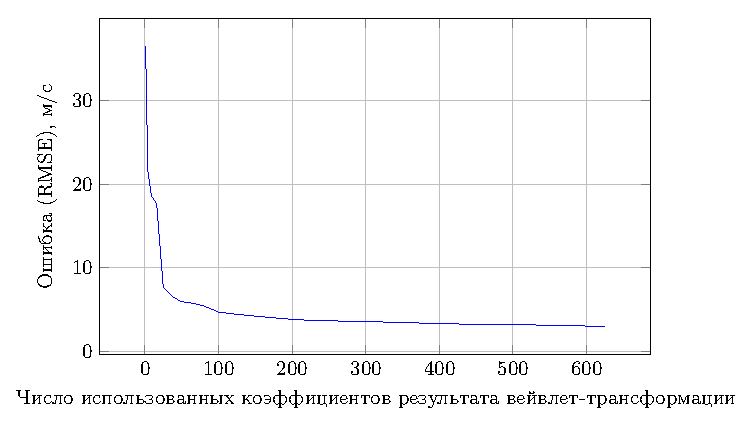
\includegraphics[width=\textwidth]{pics_eps/rmse_coef_in_use_reconstr.eps}
    \caption{\small Ошибка восстановления карты скоростей искусственной модели при использовании неполного набора коэффициентов вейвлет-преобразования.}
    \label{fig:used_coeff0}
  \end{minipage}
  \hfill
  \begin{minipage}[b]{0.8\textwidth}
    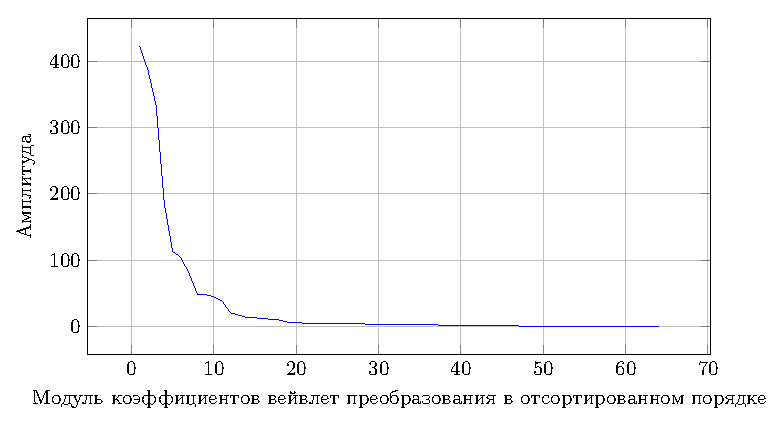
\includegraphics[width=\textwidth]{pics_eps/line_coefs_sparse_reconstr.eps}
    \caption{\small Набор коэффициентов вейвлет-преобразования.}
    \label{fig:used_coeff}
  \end{minipage}
\end{figure}

В контексте опознания со сжатием это означает, что характеристику сигнала $s$ для маломасштабной модели можно выбрать на интервале от 100 до 200 без существенной потери качества. Опираясь на отсортированный по амплитуде набор коэффициентов вейвлет преобразования (рис.~\ref{fig:used_coeff}) в дальнейшем для искусственной модели будем полагать $s=11^2 = 121 $, что составляет около $3\%$ от всех коэффициентов $N$.\\

\textbf{Анализ разреженности томографического снимка} \\

Для того, чтобы оценить влияние сложности деталей, содержащихся на изображении, рассмотрим свойства снимка, полученного при МРТ. Результаты анализа его вейвлет-преобразования представлены на рис.~\ref{fig:used_coef_mri} и ~\ref{fig:used_coef_mri2}. Таким образом для томографического снимка можем взять характеристику разреженности $s_{mri} = 25^2 = 625$, что составляет около  $3.8\%$ от размера сигнала $N=128\times 128=16384$. Результат восстановления при использовании $s_{mri}$ коэффициентов показан на рис.~\ref{fig:dwt_result_on_real}.

\begin{figure}[h]
    \centering
    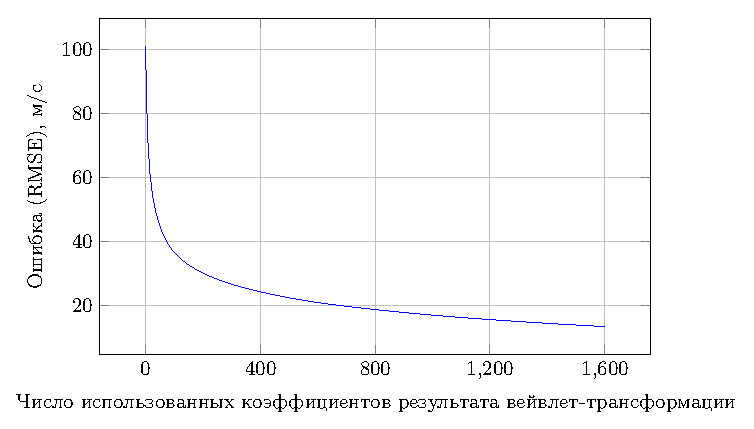
\includegraphics[width=0.8\linewidth]{pics_eps/rmse_coef_in_use_real-img.eps}
    \caption{\small Ошибка восстановления томографического снимка при использовании неполного набора коэффициентов вейвлет-преобразования.}
    \label{fig:used_coef_mri}
\end{figure}
\begin{figure}[h]
    \centering
    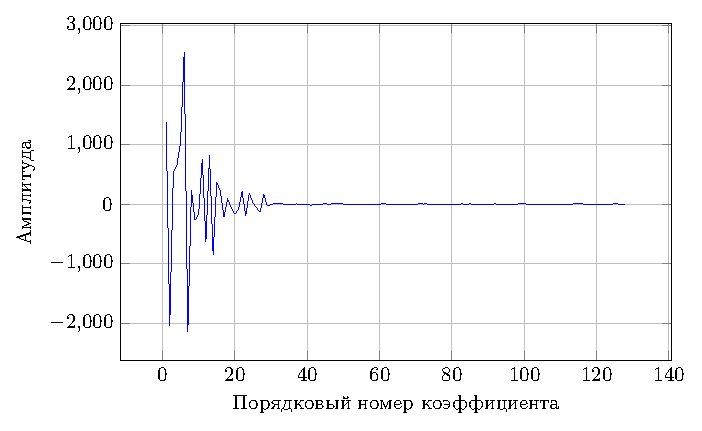
\includegraphics[width=0.8\linewidth]{pics_eps/line_coefs_sparse_real-img.eps}
    \caption{\small Набор коэффициентов вейвлет-преобразования.}
    \label{fig:used_coef_mri2}
\end{figure}



\begin{figure}[tbp]
  \centering
  \begin{minipage}[b]{0.45\textwidth}
    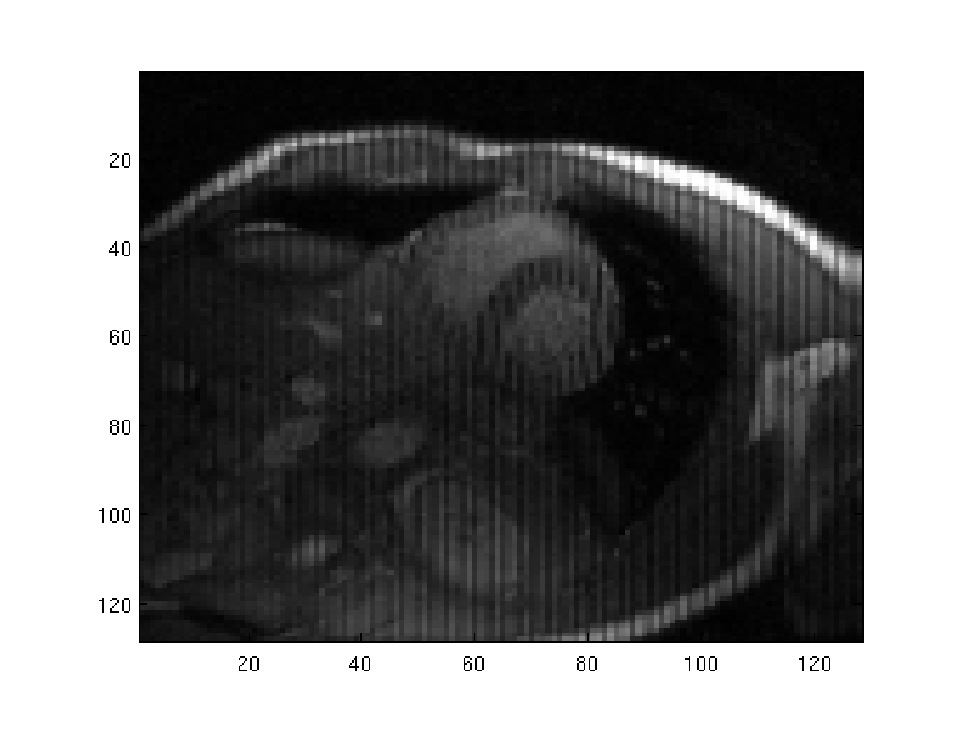
\includegraphics[width=\textwidth]{pics_eps/coef_rtv_src_img_128.eps}
  \end{minipage}
  \hfill
  \begin{minipage}[b]{0.45\textwidth}
    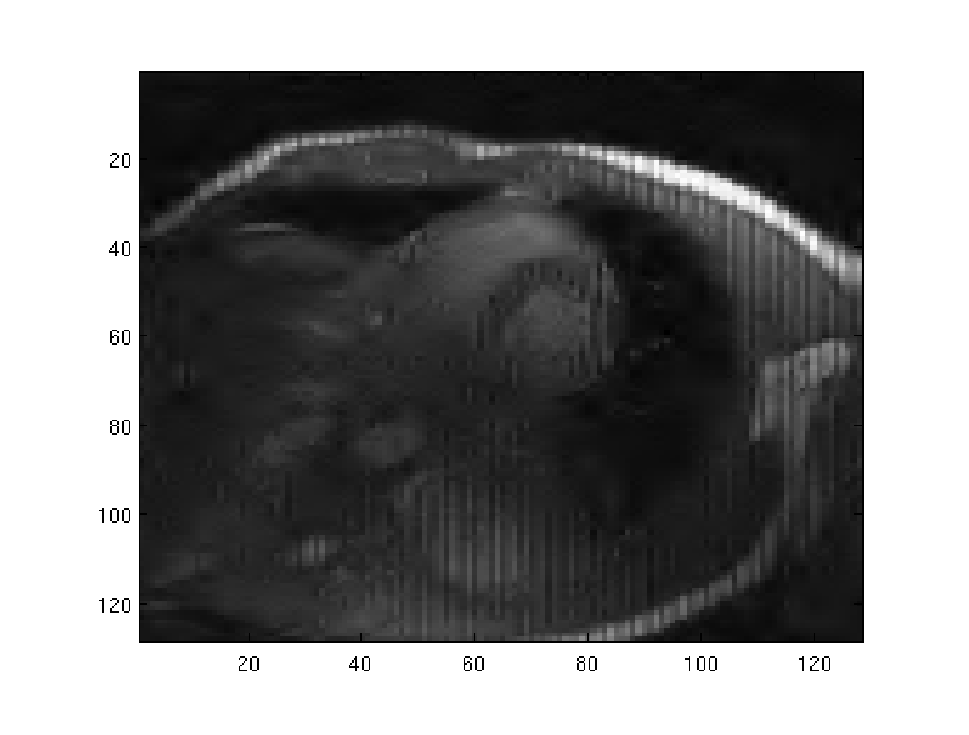
\includegraphics[width=\textwidth]{pics_eps/coef_rtv_result_img_128.eps}
  \end{minipage}
    \caption{Результат восстановления МРТ снимка при использовании $s_{mri}=25^2$ коэффициентов вейвлет-преобразования, что составляет 3.8\% от их общего объема)}
    \label{fig:dwt_result_on_real}
\end{figure}

\subsection{Ожидания по масштабированию задачи}

Характер разреженного сигнала, выражающийся параметром $s$, по большей мере зависит от сложности изображения, чем от его разрешения. Так при неизменном параметре $s$ было проведено масштабирование искусственной модели и вычислены значения среднеквадратичного отклонения (см. табл~\ref{table:problem_scaling}). Результаты показывают, что при использовании только $225$ из $2048^2$ коэффициентов вейвлет-преобразованного изображения среднеквадратичная ошибка составляет $0.16\%$ от амплитуды скоростей в изучаемой модели.

\begin{table}[h]
\centering
\begin{tabular}{ c | c | c | c | c | c | c }
    \hline
    N & $64^2$ & $128^2$ & $256^2$ & $512^2$ & $1024^2$ & $2048^2$ \\
    \hline
    RMSE, м/с & 0.0458 & 0.3131 & 0.8941 & 1.4651 & 1.6269 & 1.7754 \\
    \hline
\end{tabular}
\caption{\small Значение среднеквадратичного отклонения от длины сигнала $N$ (числа пикселей) восстановленного изображения на искусственной модели (описанной в разделе~\ref{sec:model_desc}) при характеристике разреженности $s = 15^2$. В качестве трансформирующего кодирования был использован вейвлет db6.}
\label{table:problem_scaling}
\end{table}

Это дает повод полагать, что при увеличении требуемого разрешения изображения томографической реконструкции характеристика разреженности $s$ должна увеличится незначительно, и этим фактом можно пренебречь в дальнейших теоретических оценках.\\

Можем полагать, что разрешение изображения $N \approx k^2$, где $k$ --- количество датчиков в устройстве. Тогда число уравнений, получаемых в результате максимально возможного числа проекций томографического обследования составляет \[M = k\cdot (k-1).\] Полезным результатом теории опознания со сжатием является тот факт, что для восстановления разреженного изображения достаточным является использование только $m$ измерений:
\begin{equation}\label{eq:approx_m}
m \approx 4 s  \log{\frac{N}{s}}.
\end{equation}
Так по рис.~\ref{fig:percents_est} и табл.~\ref{table:m_computed} видно преимущество, получаемое при использовании парадигмы опознания со сжатием: количество уравнений, необходимых для реконструкции требуемого разрешения, растет логарифмически по сравнению с традиционным способом использования полного набора $M$ уравнений.

\begin{figure}[h]
    \centering
    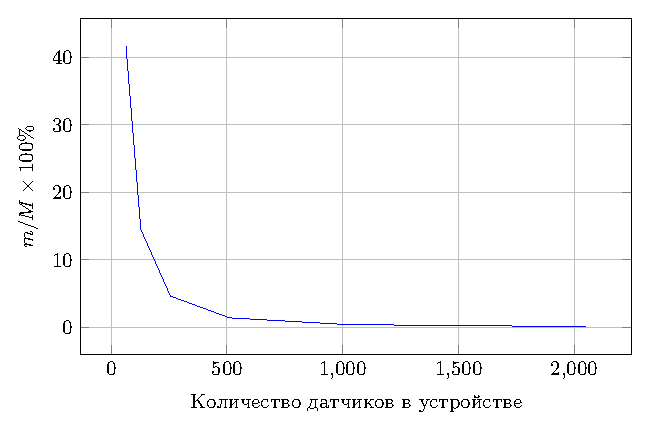
\includegraphics[width=0.8\linewidth]{pics_eps/percents_estimation.eps}
    \caption{\small Процент уравнений, достаточных для реконструкции изображения, от общего объема получаемых данных}
    \label{fig:percents_est}
\end{figure}

\begin{table}[h]
\centering
\begin{tabular}{| c | c | c | c | c | c | c |}
    \hline
    M & $64\times 64$ & $128\times 128$ & $256\times 256$ & $512\times 512$ & $1024\times 1024$  \\
    \hline
    m & 1705 & 2376 & 3047 & 3718 & 4389 \\
    \hline
\end{tabular}
\caption{\small Количество измерений достаточных для реконструкции ($m$) и полное количество произведенных измерений $M$.}
\label{table:m_computed}
\end{table}

\subsection{Проектирования универсальной матрицы измерений}
Согласно \cite{baraniuk2008simple} хороший результат дает матрица со следующим распределением элементов:
\[ A_{i,j} =
  \begin{cases}
    +\sqrt{\frac{3}{m}}      & \quad \text{с вероятностью } \frac{1}{6}\\
    0   & \quad \text{с вероятностью } \frac{2}{3}\\
    -\sqrt{\frac{3}{m}}       & \quad \text{с вероятностью } \frac{1}{6}\\
  \end{cases}
\]
Такая матрица с высокой вероятностью будет удовлетворять требованиям, описанным в разделе \ref{sec:cs_description}.\\

\textbf{Вариант 1: базовый вариант матрицы}\\

Эта же матрица будет использована для тестирования \textit{базового} метода опознания со сжатием. Это позволит сократить объем данных для последующих вычислений, однако требуется полный объем сведений о времени прибытий сигналов. Таким образом время на предварительную обработку (извлечение из измерений датчиков времени прибытия звуковой волны) не будет уменьшено.\\

\textbf{Вариант 2: равновероятный отсев данных}\\

В отличие от варианта 1, $(M-m)$ случайных столбцов матрицы будут заполнены нулями. Это далает возможным сократить также время на предварительную подготовку данных: часть датчиков может не производить измерения.\\

\textbf{Вариант 3: отсев проекций}\\

Теперь, в отличие от варианта 2, зануляться будут группы столбцов --- датчики, принявшие сигнал от какого-либо датчика, пославшего импульс. Уменьшение числа совершаемых проекций позволяет не только уменьшить объем данных для обработки, но и сократить время на непосредственно исследование пациента, что ведёт к уменьшению зашумления данных от движений тела пациента. \\

\textbf{Вариант 4: точечный выбор данных}\\

В каждой строке матрицы находится только один ненулевой коэффициент. Все ненулевые коэффициенты равны. \\

Заметим: в то время как вариант 1 опирается на полный объем данных, варианты 2,4 используют только $m \text{ из } M$ измерений. Вариант 3 округляет $m$ вверх до ближайшего значения, позволяющего использовать полное число ($k_{Rx}$) принимающих датчиков.

\subsection{Алгоритм реконструкции при использовании Com\-pres\-sive Sensing} \label{sec:recon_algo}
Реконструкция будет производиться методом сопряженных градиентов, минимизируя:
\begin{equation}
\label{eq:conj_cs}
\min_F \| \hat{A} A(F) F - \hat{A}Y \|_2^2 + \lambda \| \Psi^T F \|_1.
\end{equation}
Здесь $\hat{A}$ является одним из вариантов рандомизированных матриц измерений, в качестве $\Psi$ используется вейвлет db6, остальные переменные уже описаны в разделе \ref{sec:travel_times_descr}. 
В процессе реконструкции перемножение $\hat{A}\cdot Y$ выполняется единожды: в начале вычислений. Также произведение $\hat{A} \cdot A(F)$ можно произвести \textit{неявно}: производя вычисления матрицы путей $A(F)$ только для заведомо используемых данных. Исключением будет являться вариант-1 построения матрицы измерений $\hat{A}$, так как он использует полный объем данных.


\subsection{Архитектура программного решения}

В ходе работы было реализовано программное решение, позволяющее адаптировать алгоритм реконструкции к ультразвуковым томографам с различными характеристиками. Общая структура программы показана на диаграмме \ref{fig:software}. 

\begin{figure}[h]
    \centering
    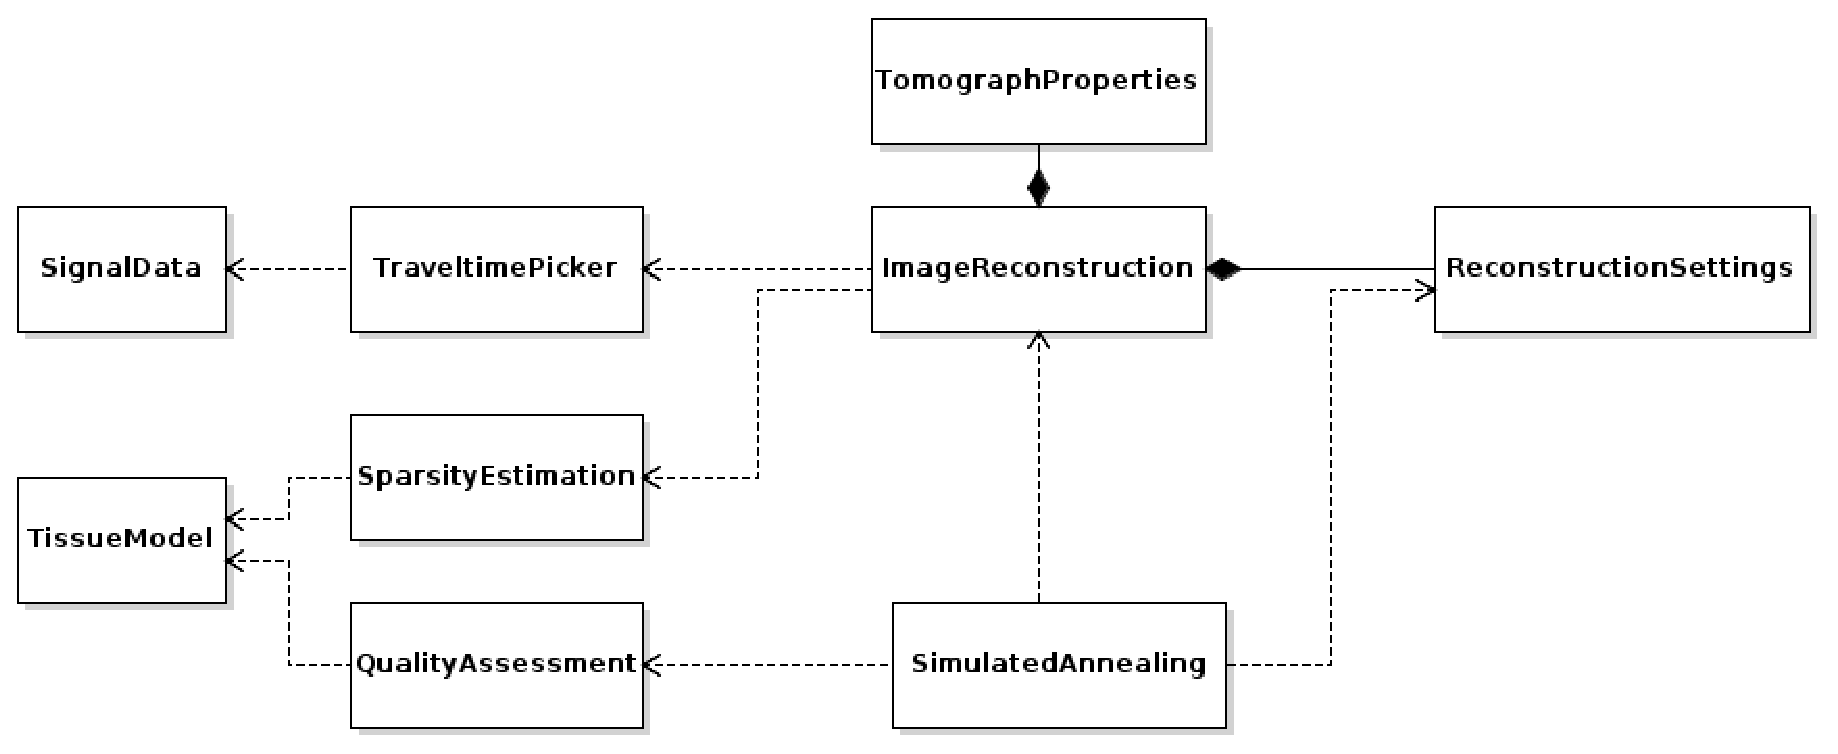
\includegraphics[width=0.95\linewidth]{pics_eps/uml_classes.eps}
    \caption{\small Архитектура программы, оптимизирующую реконструкцию томографического снимка}
    \label{fig:software}
\end{figure}

Исходными данными для программы оптимизации алгоритма реконструкция являются сущности: TomographProperties, SignalData и TissueModel. TomographProperties содержит такие характеристики томографа, как количество датчиков, диаметр кольца, на котором расположен массив датчиков. TissueModel представляет собой модель опухоли, описывающей параметры скорости распросранения звука в среде и затухания сигнала.  По модели проводится программная симуляция, результаты которой в виде записанных показаний датчиков располагаются в объекте SignalData.\\
Предварительная обработка данных заключается в извлечении из показаний датчиков времени прибытия звуковой волны. Эта нетривиальная задача решается методом, предложенным в \cite{li2009improved} сущностью TraveltimePicker. По исходной модели также необходимо определить характеристику разреженности $s$. Это происходит в SparsityEstimation посредством анализа результата вейвлет-трансформации модели с использованием модификации алгоритма First Break Picking (``STA/LTA метод''). ImageReconstruction содержит реализацию алгоритма получения снимка, описанном в разделе \ref{sec:recon_algo}. Для определения наилучших параметров алгоритма реконструкции используется метод стохастической оптимизации ``имитация отжига'', сущность SimulatedAnnealing. В качестве функции стоимости используется среднеквадратичное отклонения от заданной модели. За вычисление функции стоимости отвечает QualityAssessment. Наконец, ReconstructionSetting содержит параметры, необходимые для алгоритма реконструкции, такие как весовые коэффициенты, величину достаточной сходимости, максимальное число итераций, разрешение томографического снимка. 


\section{Моделирование} \label{sec:modeling}

\textbf{Описание маломасштабной модели} \label{sec:model_desc}

Для исследования по внедрению парадигмы опознания со сжатием в сфере ультразвуковой томографии была взята следующая модель:
\begin{itemize}
\item Исследуемая область заполнена водой. В центр помещена опухоль диаметром 5 мм.
\item Скорость прохождения звука в воде $f_w = 1500$ м/с Скорость прохождения звука через опухоль: $f_t = 2600$ м/с.
\item Диаметр кольца массива датчиков $d = 4 $ см.
\item Полное число датчиков массива, равномерно распределенных по периметру кольца: $k = 100$.
\item Число датчиков, используемых для получения сигнала, $k_{Rx} = \frac{1}{4} \cdot k$.
\item Сетка реконструкции $N = 64\times 64$.
\end{itemize}
Модель представлена на рис.~\ref{fig:model_1}.

\begin{figure}[h]
\centering
    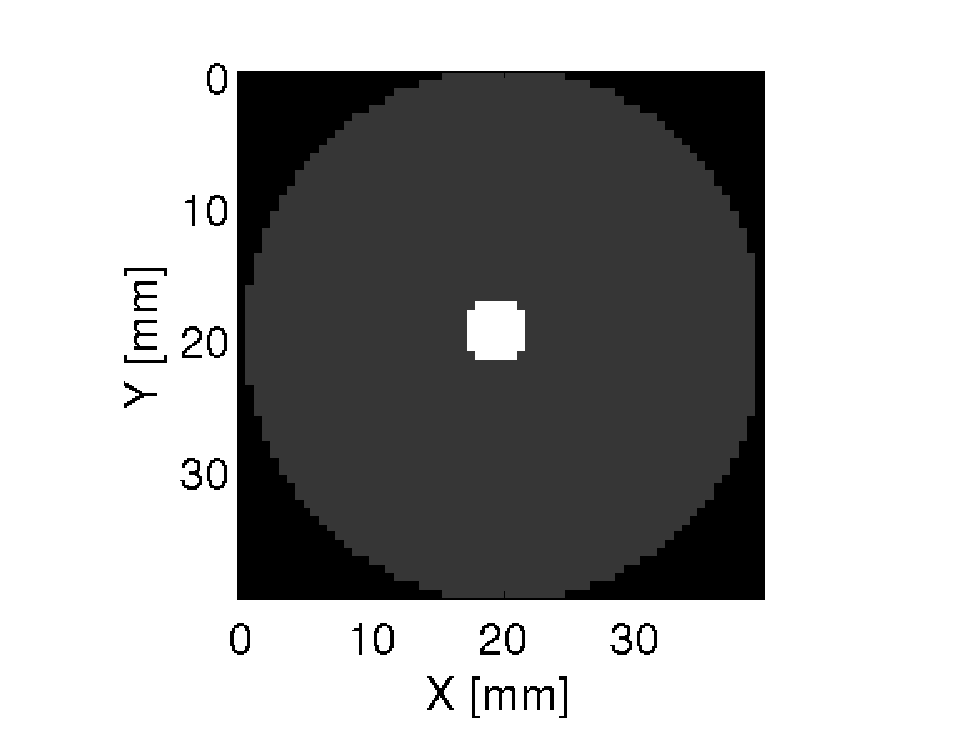
\includegraphics[width=.4\textwidth]{pics_eps/model.eps}
    \caption{\small Схема маломасштабной модели}
    \label{fig:model_1}
\end{figure}

Для симуляции модели был использован специальный инструмент для ультразвуковых исследований в среде Matlab ``K-Wave''. K-Wave неоднократно использовался в научных работах\footnote{http://www.k-wave.org/publications.php} \cite{treeby2010k}. \\


\subsection{Результаты эксперимента на маломасштабной модели}

Алгоритм реконструкции с использованием техники опознания со сжатием был протестирован на четырех вариантах построения рандомизированной матрицы измерений на 50 итерациях каждый. Результаты представлены в таблице \ref{table:fin_results}, лучшие показатели выделены шрифтом. Среди протестированных методов построения матрицы измерений лучшего результата достиг базовый вариант. Это можно объяснить тем фактом, что при построении он исходит из полного объема данных, комбинируя которые можно уменьшить влияние помех. Помехи являются неотъемлемой составляющей ультразвуковой томографии хотя бы потому, что пациент во время обследования не может быть абсолютно неподвижен. Все варианты алгоритмов с опознанием со сжатием показали лучшее качество реконструкции по метрик ``отношение сигнал-шум'' (SNR), однако по абсолютной среднеквадратичной ошибке варианты с исключением целых проекций и точечного выбора данных оказались хуже исходного алгоритма. ``Отсев проекций'' отсекает целые группы данных, что сказалось на качестве восстановления. Варианты 1--3 комбинируют различные измерения, что приводит к их большей шумоусойчивости, чего не делает вариант 4 ``Точечный выбор данных'', продемонстрировавший худшие результаты.

\begin{table}
\centering
\begin{tabular}{| l | c | c | }
    \hline
    Матрица измерений & SNR, dB & RMSE, м/с \\
    \hline
    Базовая матрица & $\mathbf{23.89 \pm 0.06}$ & $\mathbf{181.89 \pm 1.30}$ \\
    Равновероятный отсев & $23.84 \pm 0.06$ & $183.06 \pm 1.34$ \\
    Отсев проекций & $23.77 \pm 0.07$ & $184.59 \pm 1.48$ \\
    Точечный выбор данных & $23.80 \pm 0.04$ & $184.15 \pm 0.85$ \\
    \hline
    Исходный алгоритм & 23.63 & 183.36 \\
    \hline
\end{tabular}
\caption{\small Качество реконструкции снимка Compressive Sensing алгоритмами при $s = 11$  и исходным алгоритмом.}
\label{table:fin_results}
\end{table}

\begin{figure}[!tbp]
    \centering
    \begin{minipage}[b]{0.45\textwidth}
        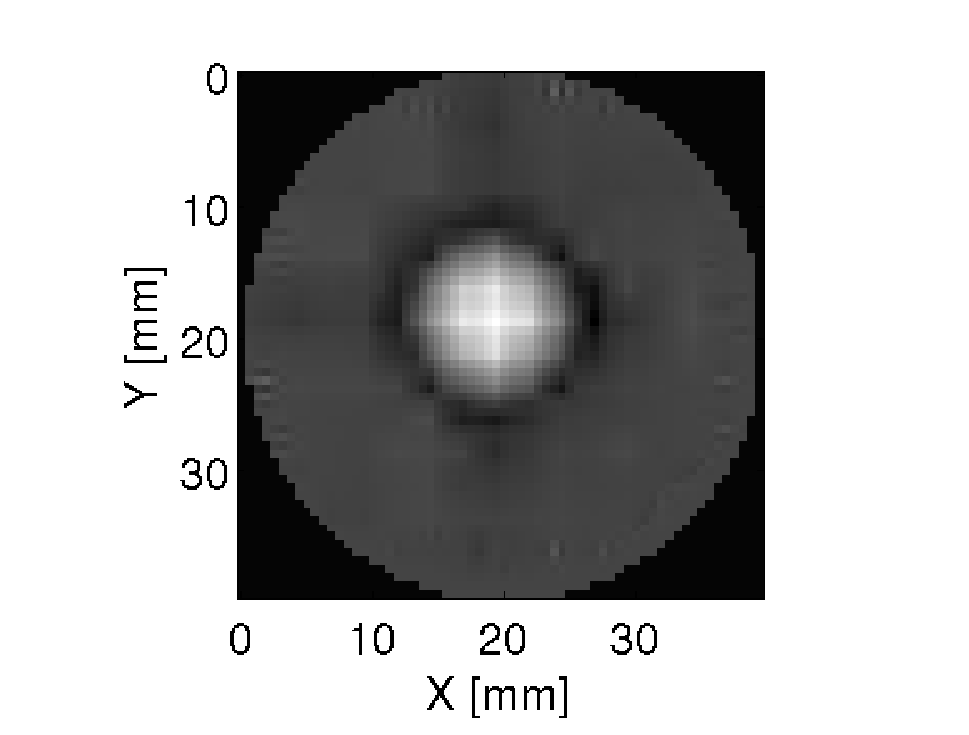
\includegraphics[width=\textwidth]{pics_eps/slice_base_grad.eps}
    \end{minipage}
    \hfill
    \begin{minipage}[b]{0.45\textwidth}
        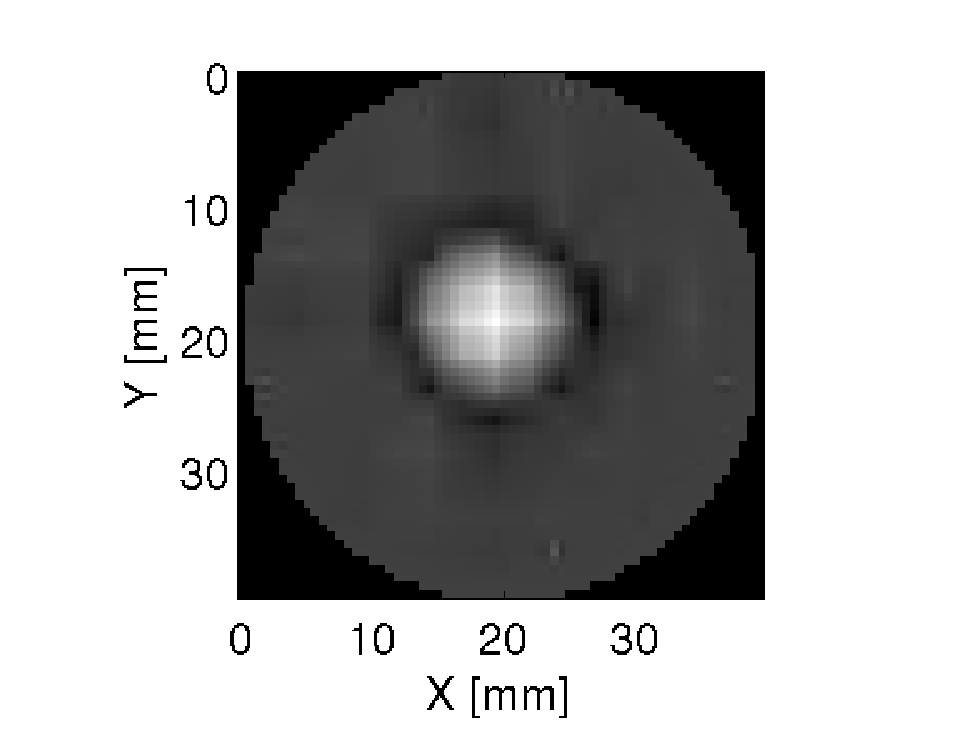
\includegraphics[width=\textwidth]{pics_eps/slice_cs_grad.eps}
    \end{minipage}
    \caption{\small Результаты реконструкции исходного алгоритма (слева) и Compressive Sensing (справа).}
    \label{fig:reconstruction_exp1}
\end{figure}


В маломасштабной модели для реконструкции можно использовать до $M = k_{Rx} \cdot k^2 = 2500$ уравнений. Повторив анализ, описанный в разделе 3.1,
%\ref{sec:s_analysis}, 
мы находим $s=11^2$.
Таким образом, применяя уравнение \eqref{eq:approx_m}, получаем достаточное для хорошей реконструкции количество уравнений $m \approx 1705$, что составляет около 68\% от общего их числа $M$. На графике \ref{fig:used_equations} отражена зависимость качества реконструкции изображения от количества исходных данных, где наилучшее значение показателя абсолютной среднеквадратичной ошибки  достигается при использовании 68-75 \% данных и в дальнейшем не претерпевает существенных изменений.

\begin{figure}[h]
    \centering
    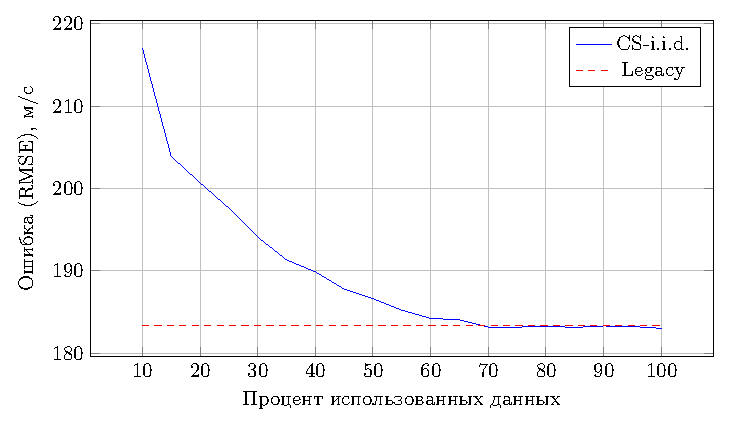
\includegraphics[width=0.8\linewidth]{pics_eps/rmse_seq.eps}
    \caption{\small Зависимость ошибки реконструкции снимка от объема использованных данных при использовании Compressive Sensing с матрицей измерений с равновероятным отсевом (CS-i.i.d.). Для сравнения показан результат исходного алгоритма, использующий полный объем данных (Legacy).}
    \label{fig:used_equations}
\end{figure}


Результаты реконструкций исходного алгоритма, используемом в ультразвуковой томографии, и Compressive Sensing представлены на рис.~\ref{fig:reconstruction_exp1}.


\section{Заключение} \label{sec:concluding}
В этой работе была исследована возможность применения техники \textit{Опознания со сжатием}, или ``Compressive Sensing'', в области ультразвуковой томографии ``времени прибытия'': изучены свойства разреженности результатов полученных изображений, а также влияние увеличения разрешения снимка на числовую характеристику разреженности $s$. Пренебрежимое увеличение этой характеристики позволяет эффективно проводить обработку данных, даже при увеличении их исходного количества на много порядков. \\
Также была разработана и апробирована на искусственных моделях модификация алгоритма реконструкции томографических снимков с применением техники опознания со сжатием. Эксперименты показали, что возможна реконструкция изображения без существенной потери качества при использовании неполного объема данных. Кроме того, некоторые варианты построения матриц измерений продемонстрировали положительное влияние на шумоустойчивость алгоритма.

% \begin{equation}
% \min_F  \sqrt{\displaystyle\sum_{i=1}^{M} (\displaystyle\sum_{j=1}^N | A_{i,j}F_i - Y_i |^2)}
% + \lambda \displaystyle\sum_{i=1}^N (\displaystyle\sum_{j=1}^N| \Psi_{i,j} F_i|)

% \end{equation}

% ----------------------------------------------------------------------------------


\setmonofont[Mapping=tex-text]{CMU Typewriter Text}
\bibliographystyle{ugost2008ls}
\bibliography{diploma.bib}
\end{document}
